\section{Monocular SLAM}
    \begin{frame}{Monocular SLAM}
        \textbf{PTAM - Parallel Tracking And Mapping}
        \vspace{-0.5cm}
        \fig{0.8}{ptamtracking}
        \vspace{-0.7cm}
        Measurements are not metric.
    \end{frame}
    \note{
        \vspace{-0.5cm}
        I will now try to present in slightly more detail some of the main areas of the thesis.

        For the video based SLAM part of this thesis, a library called PTAM was used.
        PTAM - short for Parallel Tracking And Mapping - is developed at
        Oxford University for research and use in the field of Augmented Reality.
        Again, the idea is to track features, here shown as dots, through
        the video frames to estimate the camera's position.
        Often, stereo vision is applied to extract depth information from the recorded scene.
        With monocular SLAM however, the movement of the features need to be tracked
        to extract the depth of each feature in the image.

        One major problem with video based tracking is that, unless you know something
        about the recorded scene, there is really no way of knowing wether its a large scene
        that moved a lot, or a small scene that just moved a little.
        As for instance when you film a dollhouse, there is simply no way
        to tell it from a real house, and yet the scale of movement is completely different.
    }
    \begin{frame}{Camera Measurements}
        \textbf{Measurement: } Pose relative to PTAM coordinate system.
        \vspace{-0.4cm}
        \begin{figure}[H]
        \centering
            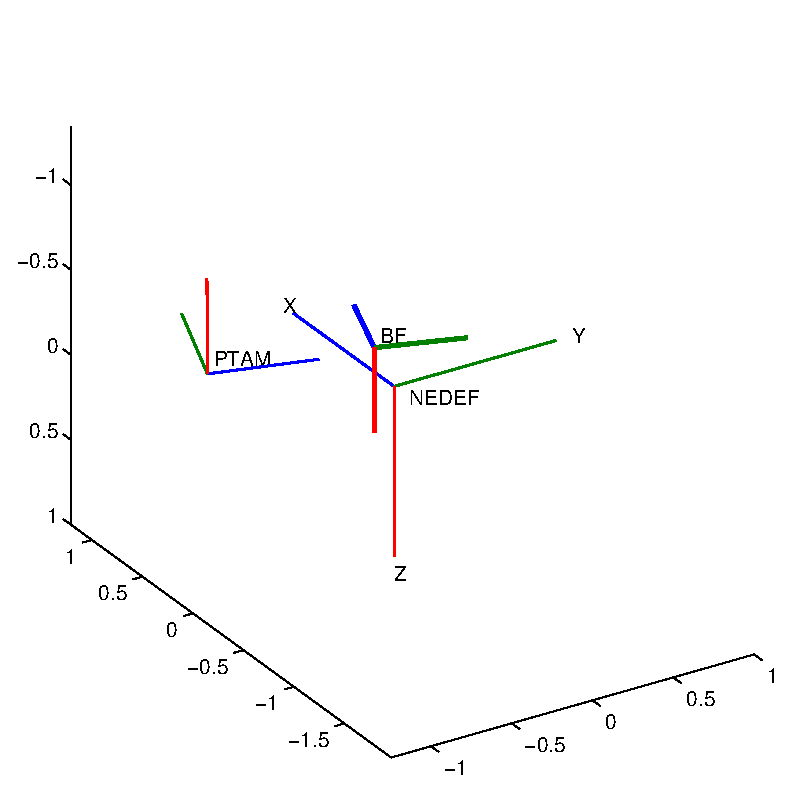
\includegraphics[trim = 0mm 0mm 0mm 20mm,clip,width=0.5\textwidth]{\currentchapter/figures/worldcoordframes}
        \end{figure}

        \vspace{-1cm}
        %~ The PTAM library is intended for use in Augmented Reality, AR.
        \begin{itemize}
            \item PTAM's coordinate system is quite arbitrarily initialised.
            \item Rotation and translation are measured in the local PTAM coordinate system.
            \item Its relation to the world must be established.
        \end{itemize}
        %~ \begin{itemize}
            %~ \item Intended to be used with wide-angle lens.
        %~ \end{itemize}
     % Intended for AR applications.
     % Intended for use with wide-angle camera lenses
    \end{frame}
    \note{
        Since the PTAM library is oblivious of the scale, this
        needs to be extracted from other sources, and autonomously so since
        the PTAM coordinate system is initialized quite arbitrarily.

        This coordinate system is of central importance, since all measurements
        are given in it, and yet both orientation, position and scale is initially unknown.
        This transformation needs to be determined before the measurements are of much use.
        In the thesis, I propose a routine to extract this transformation.
    }


    \subsection{Initialization}
    \begin{frame}{Initialization}
        PTAM tries to initialize its coordinate system on ground plane.
        %~ \vspace{-2cm}
        %~ \fig{0.7}{ground}
        \vspace{-0.5cm}
        \begin{figure}[h]
        \centering
            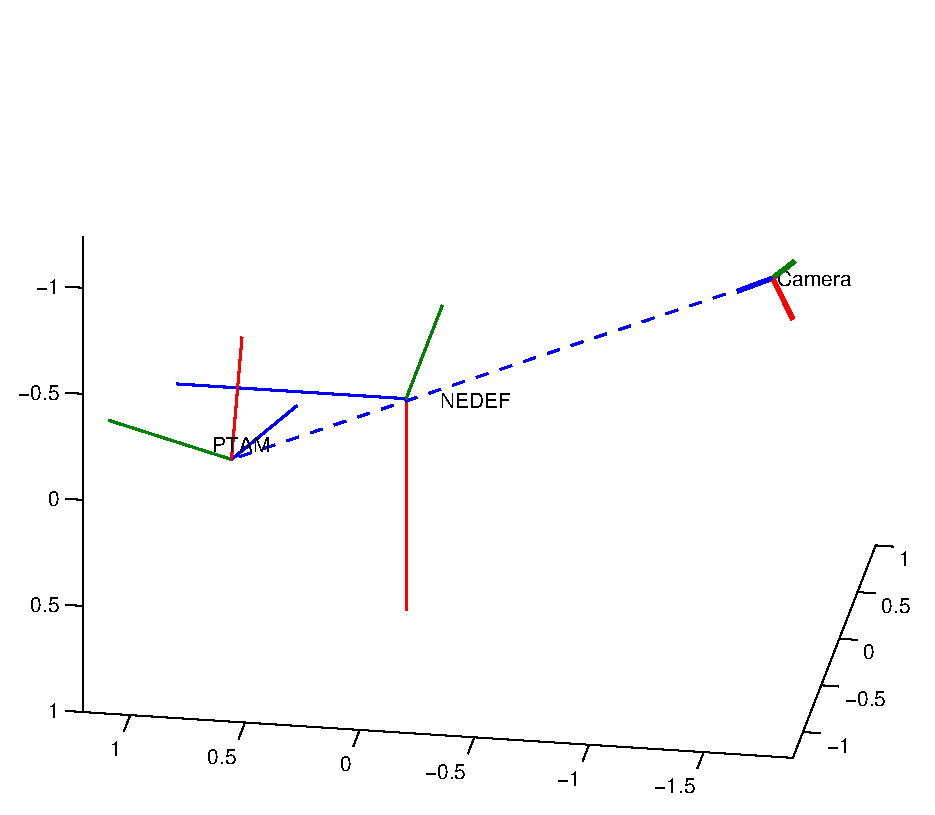
\includegraphics[trim = 0mm 0mm 0mm 20mm,clip,width=0.6\textwidth]{\currentchapter/figures/ground}
        \end{figure}

        \vspace{-1cm}
        \begin{align*}
            \left\lbrace
            \begin{array}{ll}
                \varnothing_{\text{PTAM}} &= \xi + R(q^{wb}) r_{\text{camera}/\mathcal{G}} + \lambda R(q^{wP}) \frac{X^{PTAM}}{|X^{PTAM}|} \\
                \varnothing_{\text{PTAM}} \cdot \hat{z} &= 0
            \end{array}\right. \\
        \end{align*}
        %~ \begin{equation*}
            %~ s = \frac{|X^{PTAM}|}{|\lambda|}
        %~ \end{equation*}
    \end{frame}
    \note{
        In its initialization, PTAM tries to place the coordinate system on the ground plane.
        Knowing our position of initialization, we can calculate backwards
        from the first measurement and make a guess of the position and
        orientation of the coordinate system.

        This is done by solving a system of equations and comparing the
        measured data to what was actually expected from the assumptions
        of the surroundings.

        The initialization process proposed in the thesis takes into account
        the position of the vehicle, its orientation and the camera's
        estimated distance to the ground plane in the direction
        suggested by the measurement.
    }

    \subsection{Connecting the Coordinate Systems}
    \begin{frame}{Camera Measurements}
        To extract positioning measurements usable in the real world,
        the coordinate systems have to be related.
        \begin{align*}
            x^{\text{PTAM}} &= S(s) R(q^{Pw}) T(-\varnothing_{\text{PTAM}}) x^{\text{NEDEF}} \\
            q^{PTAM,c} &= q^{Pw} q^{wb} q^{bc}
        \end{align*}
\vspace{-1cm}
        \begin{itemize}
            \item Describes the measurements in terms of the estimated state and known transformations.
            %~ \item Measurement equation for the state estimation.
        \end{itemize}
\vspace{-0.5cm}
        \begin{figure}[h]
        \centering
            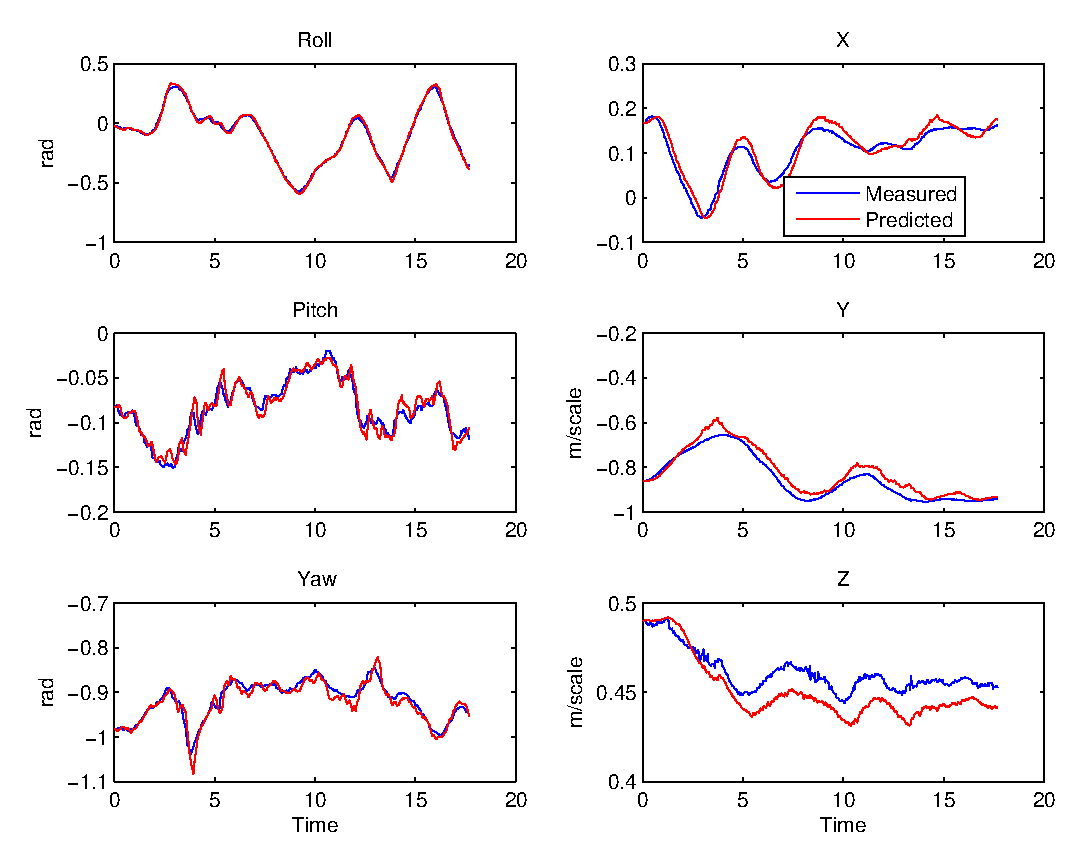
\includegraphics[trim = 0mm 50mm 0mm 0mm,clip,width=0.6\textwidth]{\currentchapter/figures/camera}
        \end{figure}
    \end{frame}
    \note{
        This transformation can then be used to connect the incoming
        measurements to the state estimation framework,
        by expressing the measurements in terms of the available states and constants.

        As seen in the image, the described transformation from the filtered position
        corresponds to the camera measurements with high precision.
    }

    %~ \subsection{Library Modifications}
    %~ \begin{frame}{Library Modifications}
        %~ In a deployment environment, the initialization and utilization of
        %~ the camera sensor must be autonomous.
%~
        %~ In the thesis, several changes are implemented to the PTAM library, e.g.
        %~ \begin{itemize}
            %~ \item Autonomous initialization procedure,
            %~ \item Re-initialization,
            %~ \item Origin positioning error detection,
            %~ \item Remote interface for non-GUI use.
        %~ \end{itemize}
    %~ \end{frame}
    %~ \note{
        %~ I mentioned earler that several changes were needed to the PTAM
        %~ library for it to work fully autonomously, and without the use of
        %~ a graphical interface.
    %~ }
